\section{User Study}
\subsection{Introduction}

To validate the usefulness of our system we decided to conduct a Within-Subjects User Study. The user study was designed to show the capacity of the system for being used in research. The study was designed to test the effectiveness of users using volumetric displays under different conditions.

\subsection{Experimental Variables}

For this study we wanted to evaluate the difference in performance of participants in interacting with volumetric screens directly with their hands vs via teleoperation. 

Our two independent variables which we varied over the study were: 
\begin{itemize}[itemsep=-0.25em]
	\item \textbf{3D Perspective}: (On/Off). This controls if the system is able to use the eye tracking system to create the illusion of a 3D volumetric display as opposed to a fixed perspective on a standard monitor as can be seen in Fig~\ref{fig:direct-vs-offset}.
	\begin{figureBox}[label={fig:direct-vs-offset}, width=0.8\linewidth]{Direct \& Offset Interaction}
		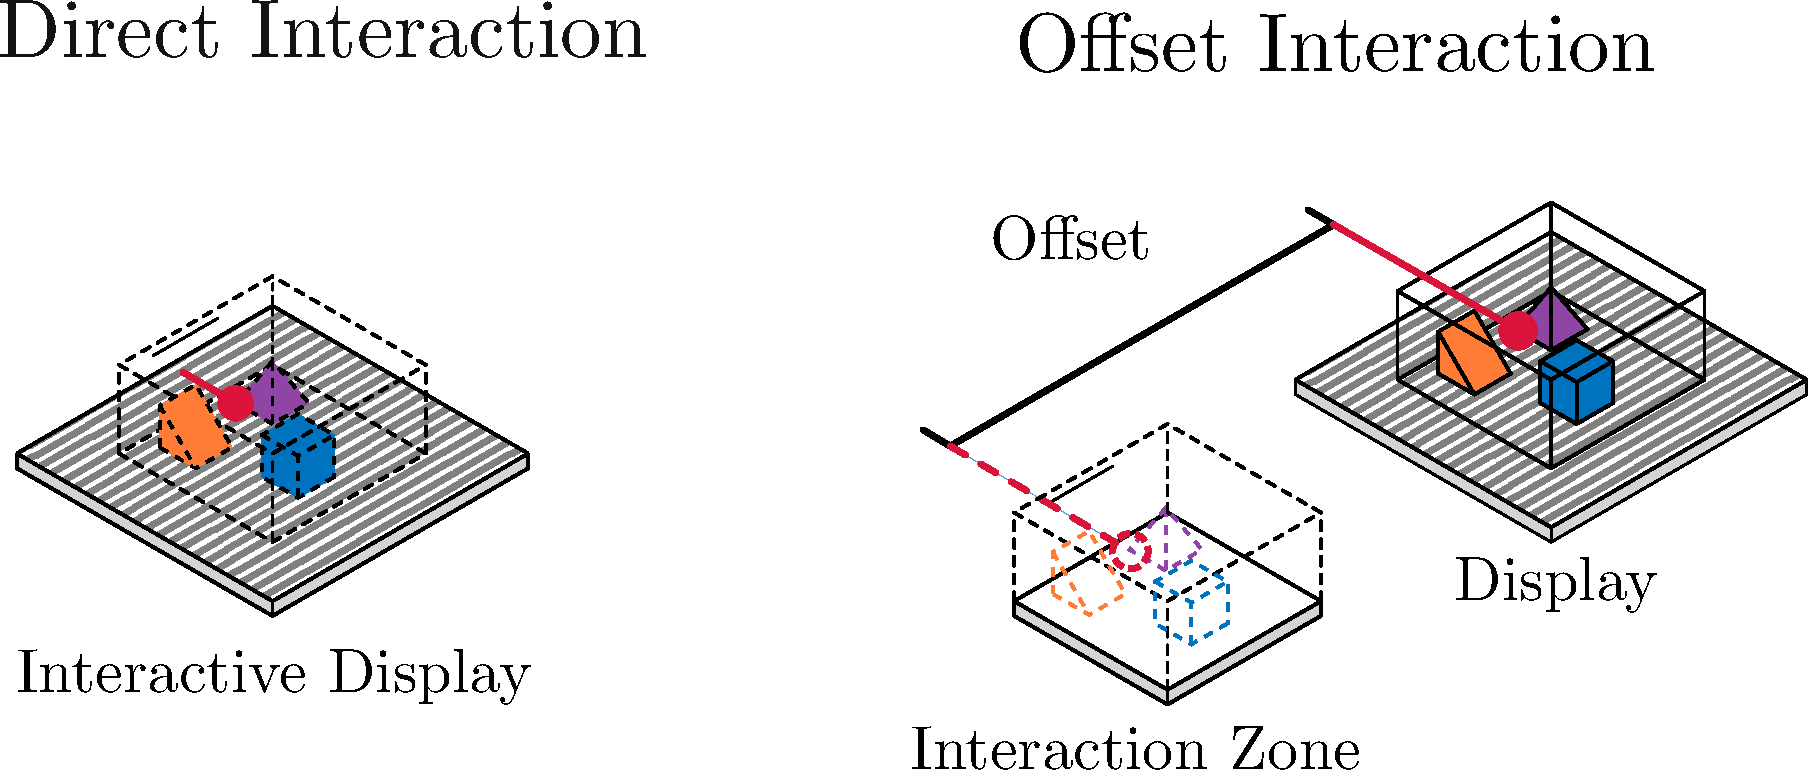
\includegraphics[width = 0.8\linewidth]{./implementation/figures/direct-vs-offset.pdf}
	\end{figureBox}
	\item \textbf{Interaction Offset}: (On/Off). This controls if display is directly in front of the participant or if it is offset by a fixed amount as can be seen in Fig~\ref{fig:2D-vs-3D}.
	\begin{figureBox}[label={fig:2D-vs-3D}, width=0.8\linewidth]{2D \& 3D}
		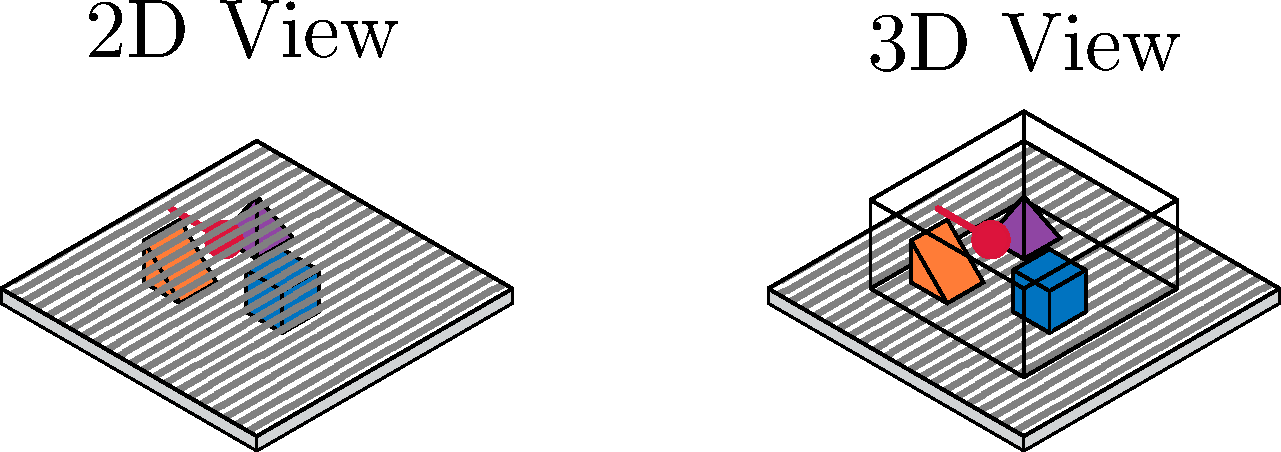
\includegraphics[width = 0.8\linewidth]{./implementation/figures/2D-vs-3D.pdf}
	\end{figureBox}
	
\end{itemize}

We made sure to control for the following variables: We made sure that the five tasks were the same in each condition. We also made sure that the position of the participant, the tracking camera, and the zone of interaction were the same in each condition as can be seen in Fig~\ref{fig:test-setup}. We were careful to ensure the lighting conditions inside the room did not change. When using an offset position we placed another display where the old display was to ensure tracking was consistent.

\begin{figureBox}[label={fig:test-setup}, width=0.8\linewidth]{Test Setup}
    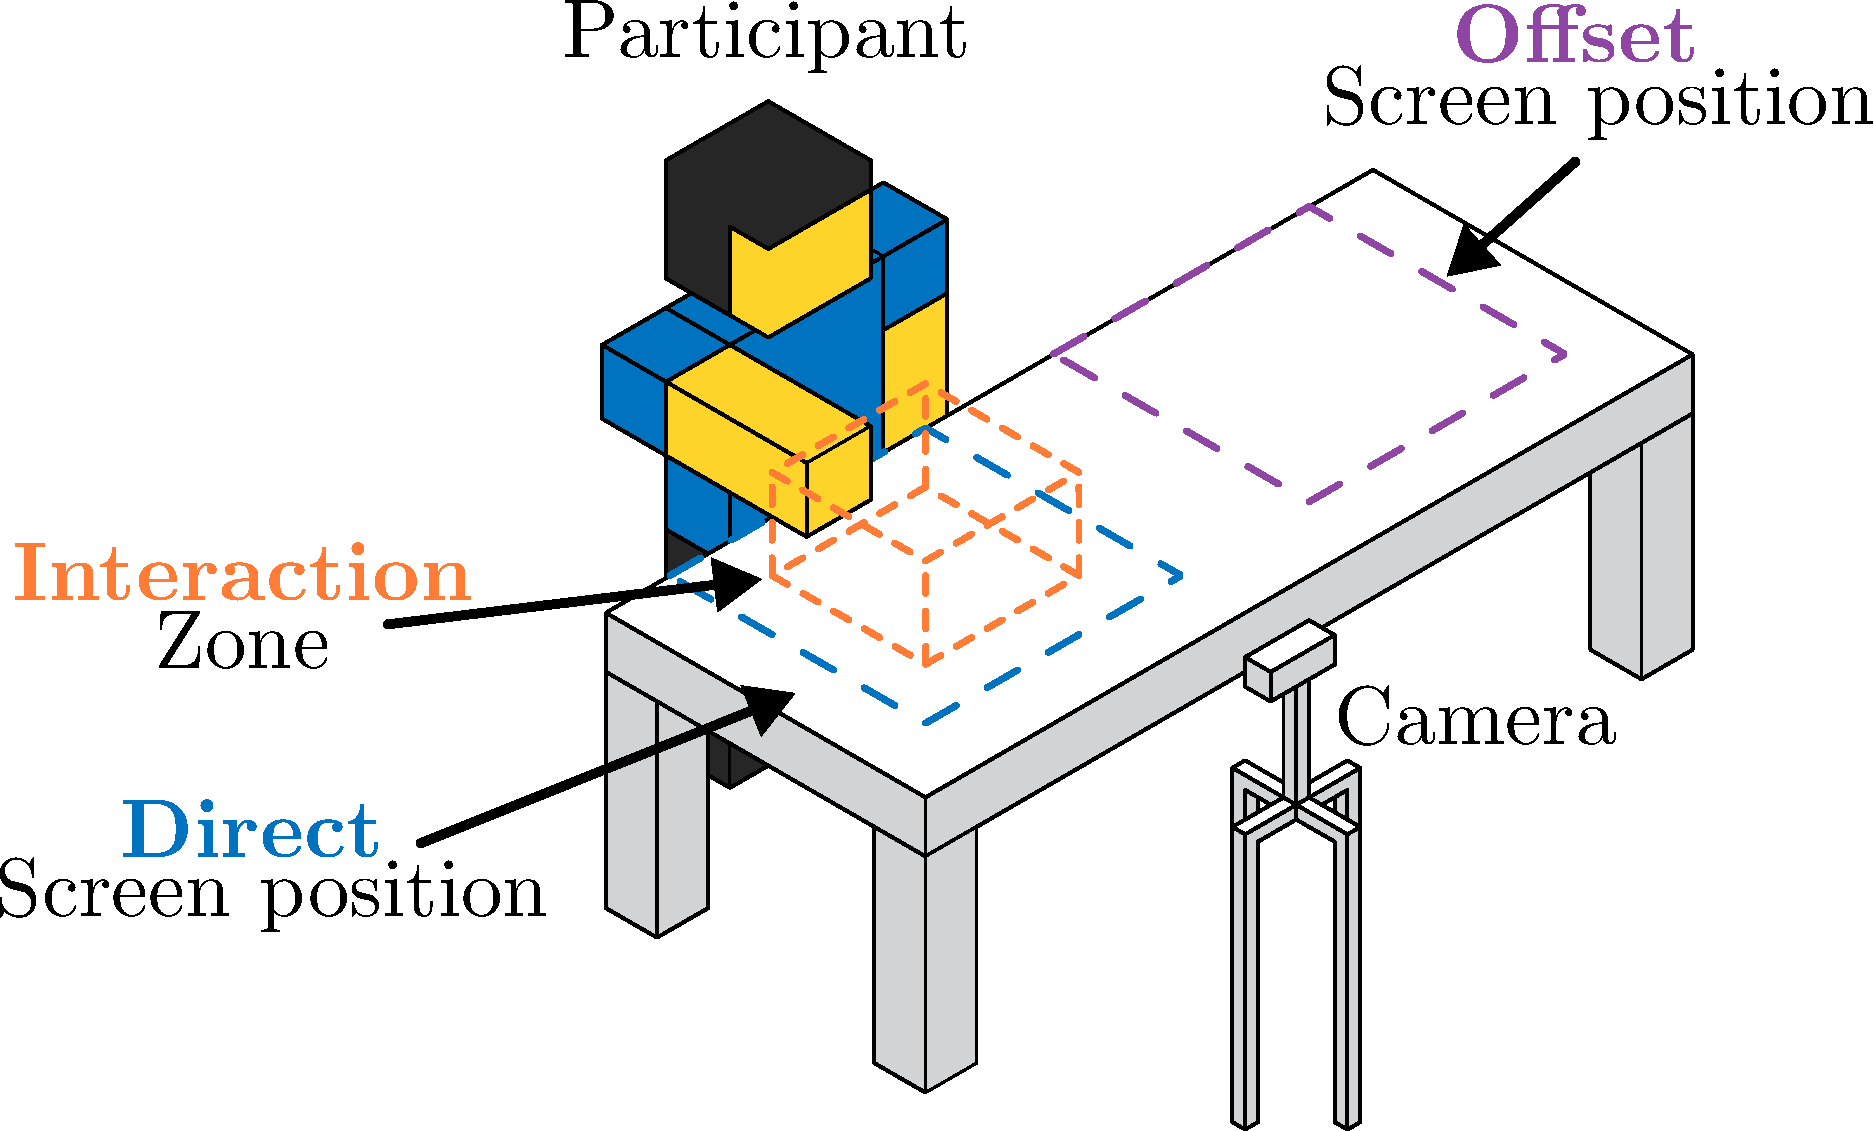
\includegraphics[width = 0.8\linewidth]{./implementation/figures/test-setup.pdf}
\end{figureBox}

\subsection{Tasks}
In each of the 4 conditions the participant must complete the same 5 tasks. The tasks are designed to be simple but more difficult to complete if not in 3D. To complete a task a participant must trace the path between the points with their index and middle finger in the order the simulator presents to them. A green point is completed segment, an orange point represents the next point to be completed and a red point in the current position of the participants hand as can be seen in Fig~\ref{fig:test-setup}. \\ 

\begin{figureBox}[label={fig:task-example}, width=0.8\linewidth]{Completing a task}
    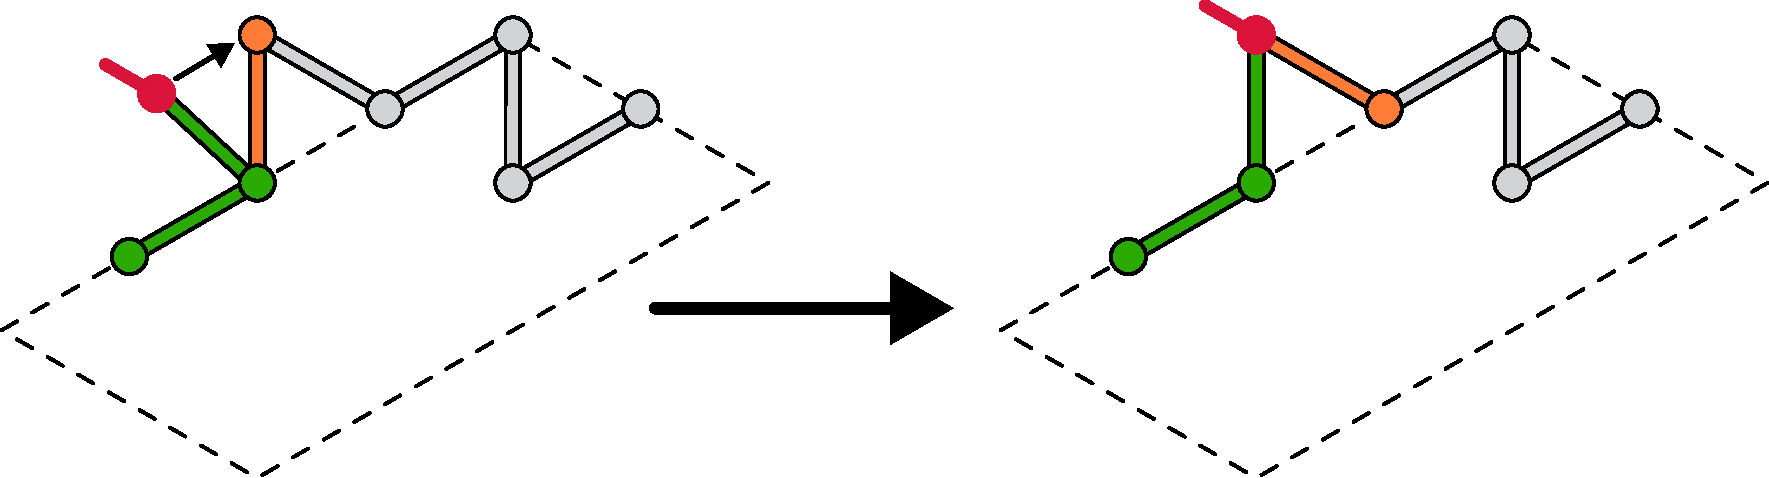
\includegraphics[width = 0.8\linewidth]{./implementation/figures/task-example.pdf}
\end{figureBox}

The participants have a timeout of 1 minute to complete the task. If they do not complete the task in the time limit, the task is marked as incomplete. The time each point is completed is recorded as well as the position of the hand and eye throughout the minute. The 5 different tasks are shown in Fig~\ref{fig:tasks} The participants are also given two demo tasks to get used to the system. \\

\begin{figureBox}[label={fig:demo-conditions}, width=0.8\linewidth]{Demo Conditions}
    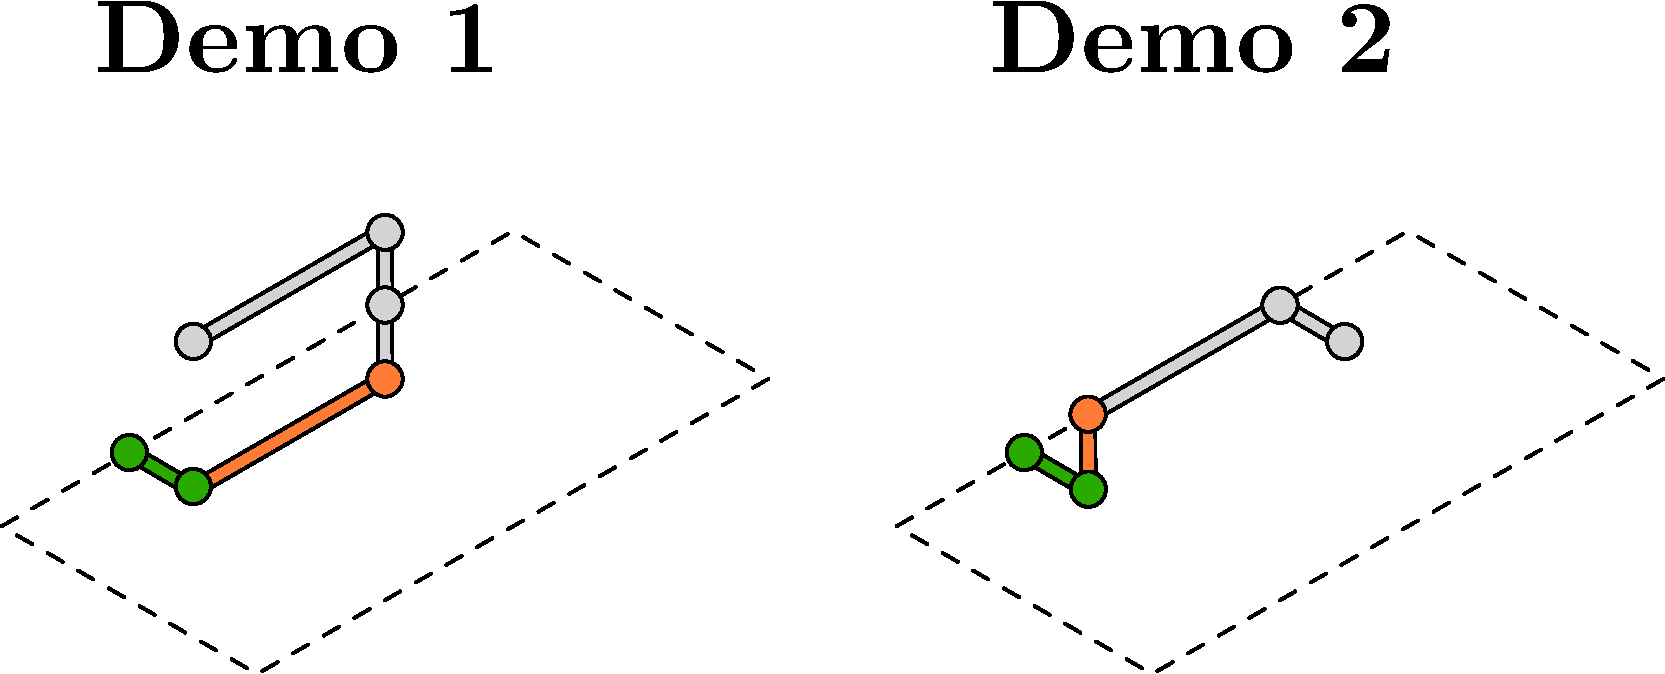
\includegraphics[width = 0.65\linewidth]{./implementation/figures/demos.pdf}
\end{figureBox}


\begin{figureBox}[label={fig:tasks}, width=1.0\linewidth]{The 5 tasks}
    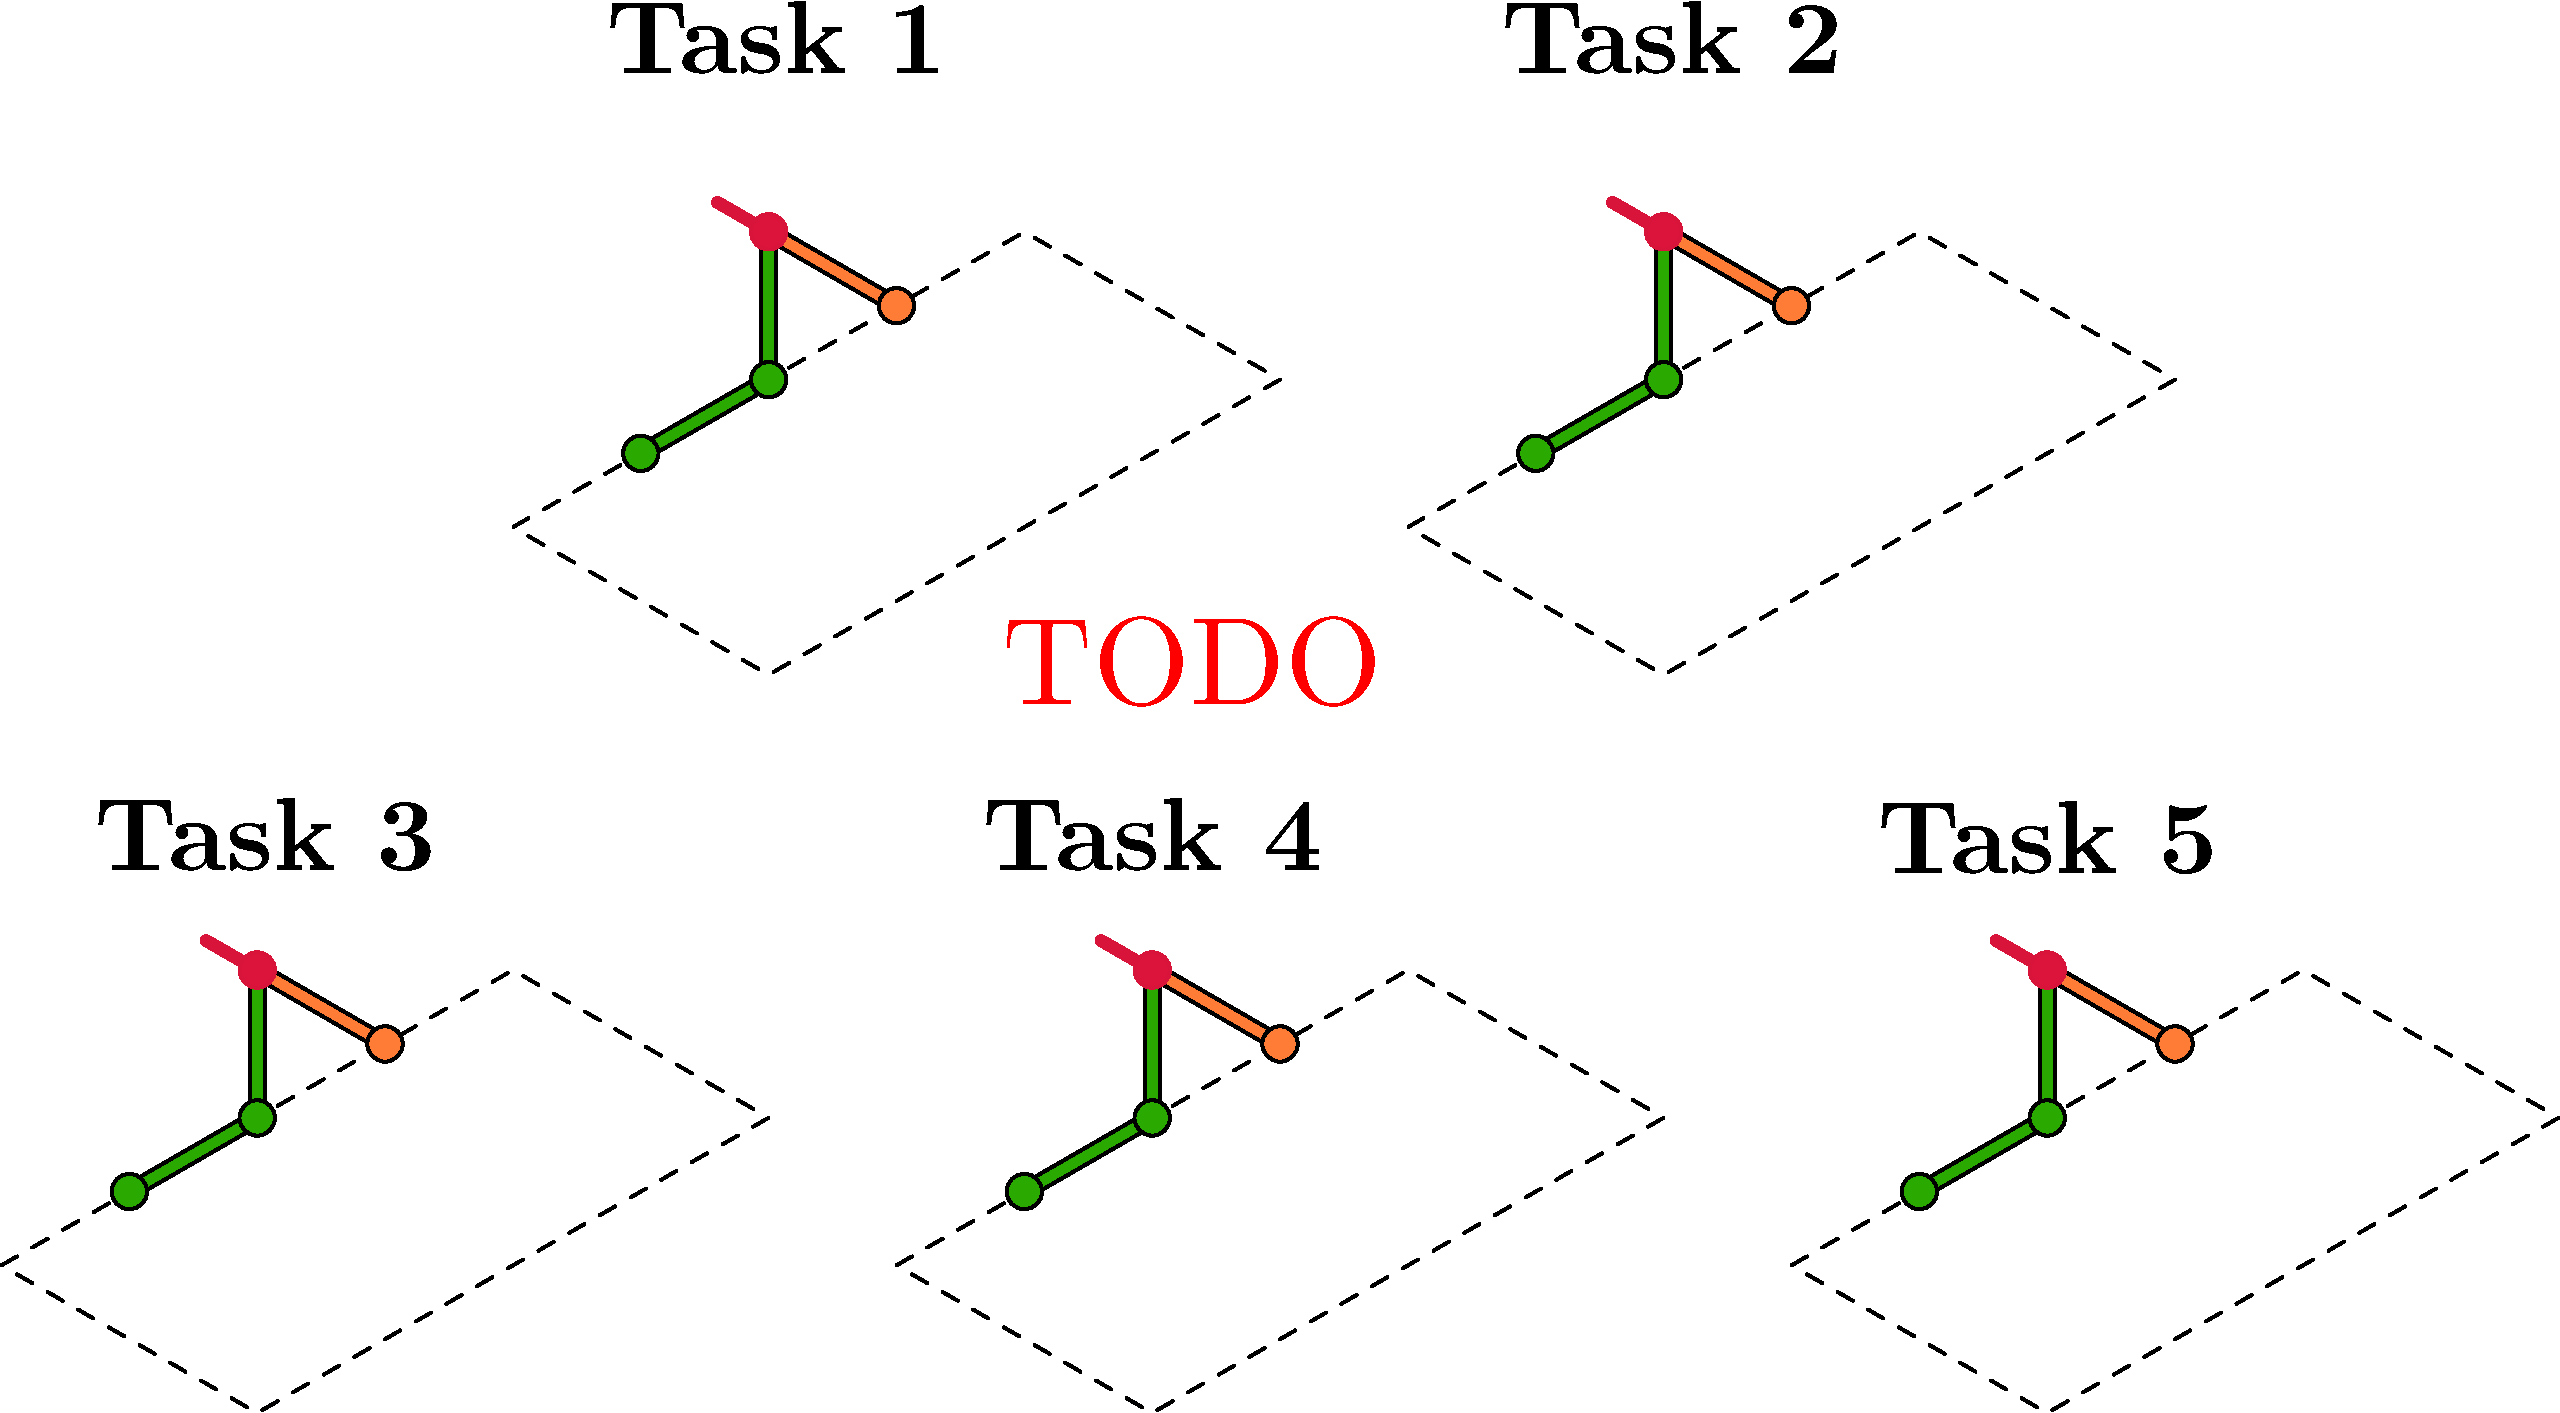
\includegraphics[width = 0.8\linewidth]{./implementation/figures/tasks.pdf}
\end{figureBox}

\subsection{Participants}
We invited participant to take part in the study via email and text using a standardized script. On arrival the participants were asked to fill out a consent form and a questionnaire about themselves to find out information that might affect the results, such as their age, handedness and previous experience with VR/AR. \\   

They were next given a brief overview of the system and allowed to run through two demo tasks in each of the 4 different configurations to get used to the system. They were advised to keep their non-dominant hand on their lap, and place their dominant hand on the monitor face down at the beginning of each task to aid with tracking. They were allowed to do this up to three times.\\

When they were comfortable with the system they were entered into our system and were automatically assigned a random order of the four conditions that can be seen in Fig~\ref{fig:study-conditions}. 

\begin{figureBox}[label={fig:study-conditions}, width=0.8\linewidth]{Study Conditions}
    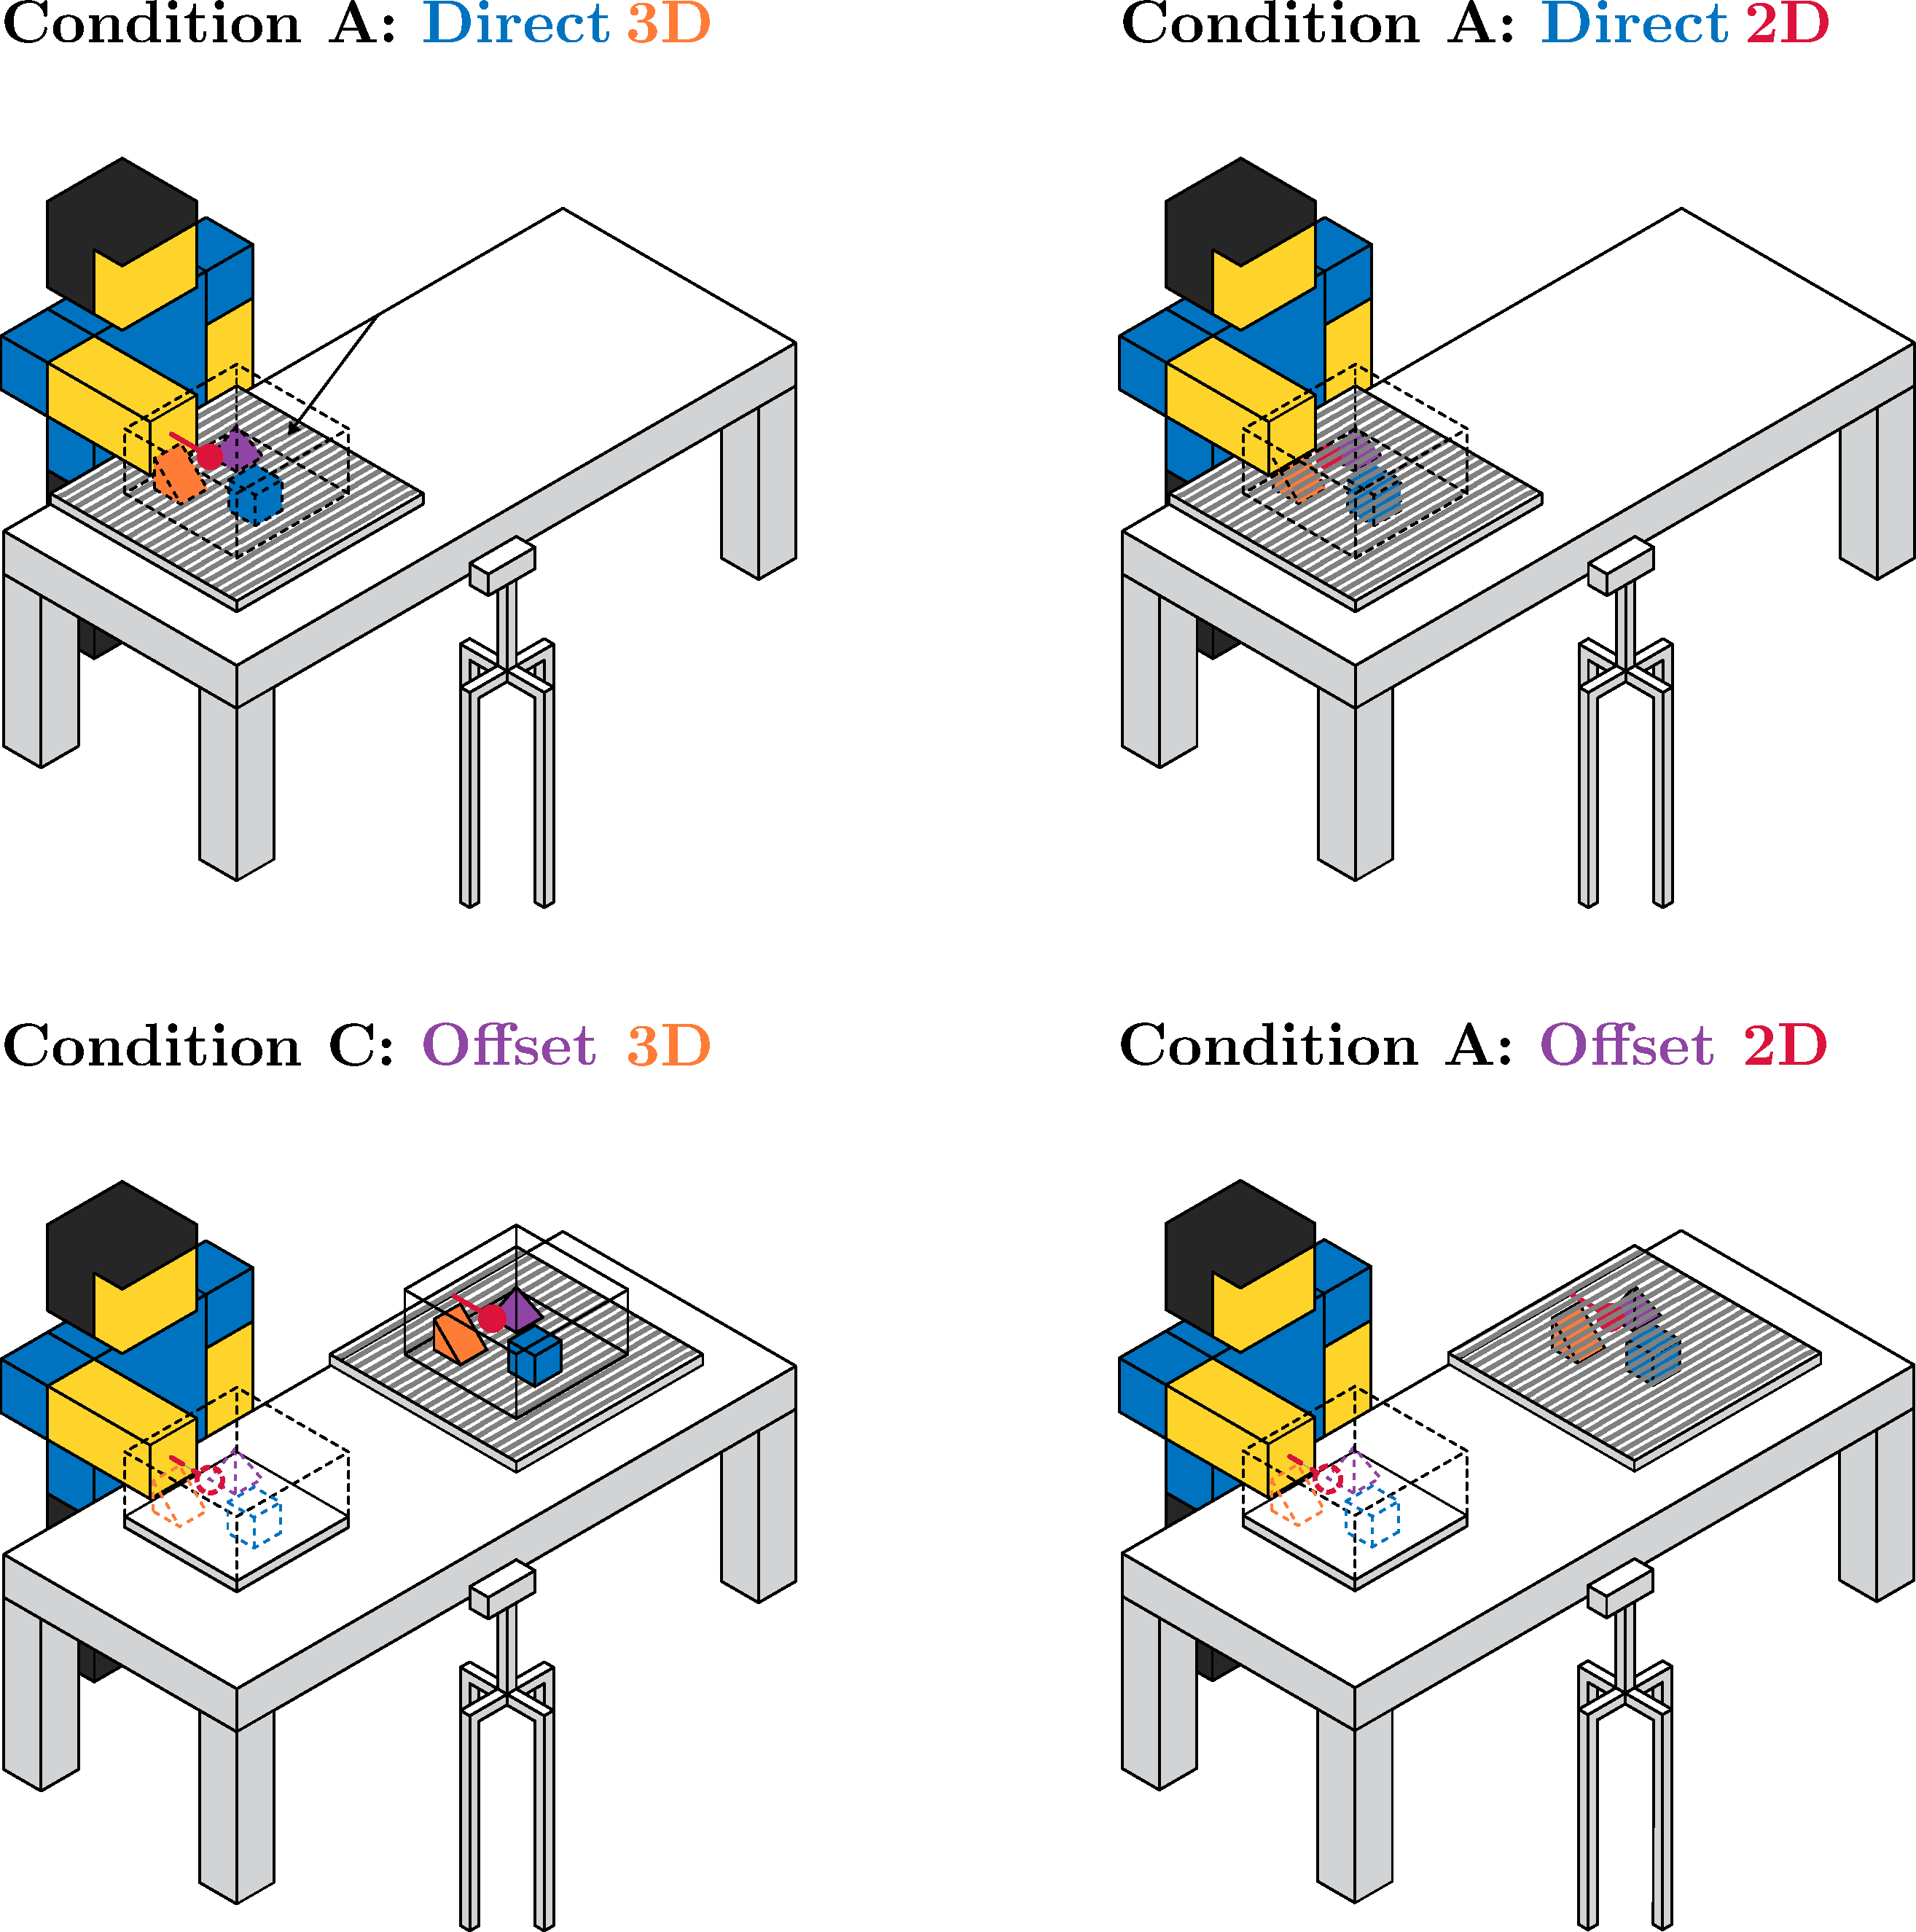
\includegraphics[width = 0.8\linewidth]{./implementation/figures/study-conditions.pdf}
\end{figureBox}

Each condition consisted of the 5, 1 minute tasks that the participants had to complete in order. They were given an audio cue when the task was about to start and when it had finished. The participants were allowed to take breaks between conditions. After each condition they were asked to fill out a survey about the condition. At the end of the study they were asked to fill out a survey about the system as a whole. 

\subsection{Setup}

The study was run on the groundfloor of the Huxley building in Room 218 at Imperial College London. As we knew we would be conducting the study over multiple days, we made care to set up the system in such a way it would be difficult to tamper with. As can be seen in Fig~\ref{fig:front-view-study} we put our camera on a tripod and marked the positions of the legs on the floor. We also surrounded the camera with a barrier of tables to prevent it from being knocked over. \\

\begin{invisBox}  
	\pictureBox[label={fig:front-view-study}]{Study: Front View}{
	  \adjustbox{height=5cm, keepaspectratio}{
		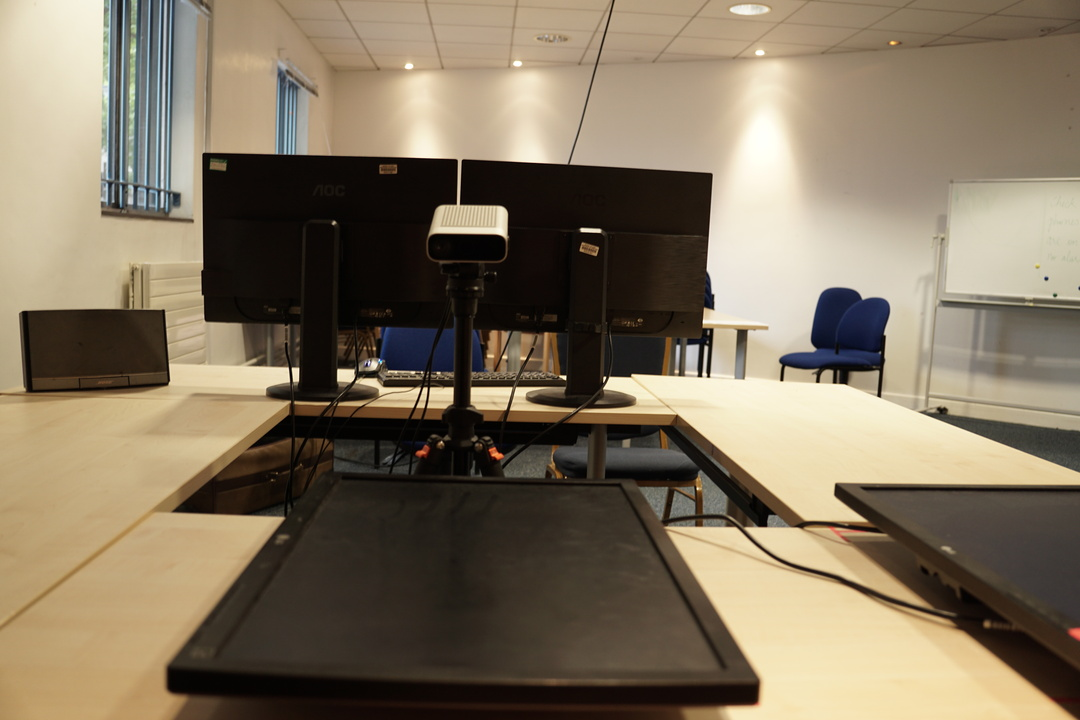
\includegraphics{./implementation/figures/front-view.jpg}
	  }
	}
	\hfill
	\pictureBox[label={fig:side-view-study}]{Study: Side View}{
	\adjustbox{height=5cm, keepaspectratio}{
	  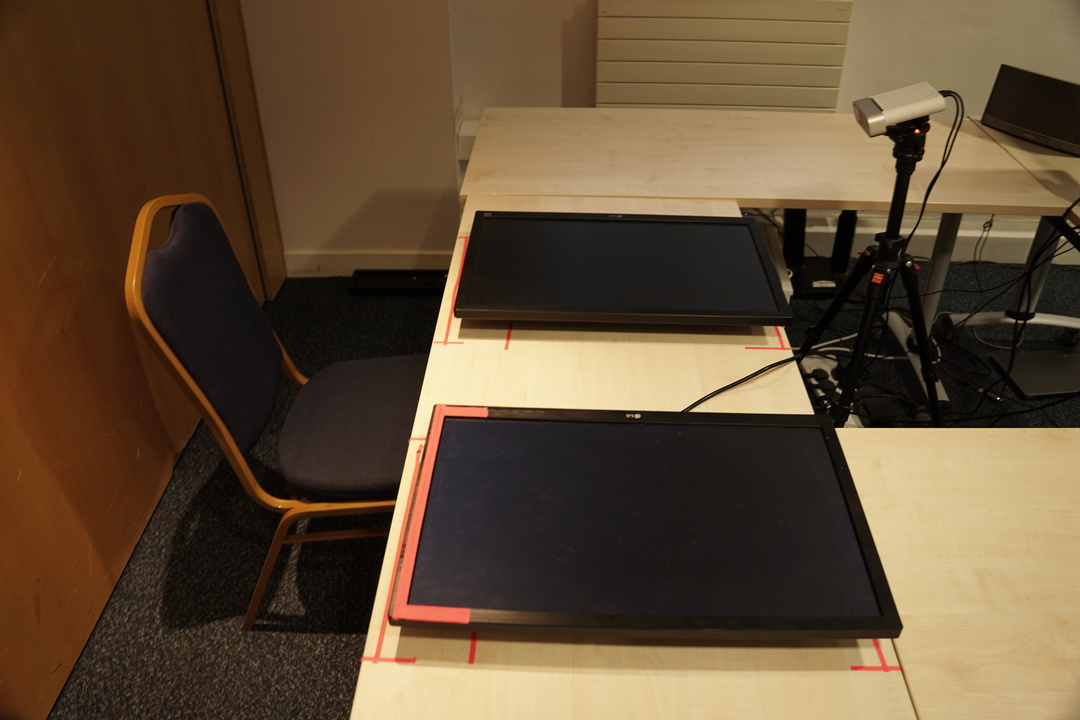
\includegraphics{./implementation/figures/side-view.jpg}
	  }
	}
\end{invisBox}

The displays we used for the study were $24''$ $1920 \times 1200$ $\texttt{LG IPS LED 24EB23}$ computer monitors that we had taken off the stands and places horizontally on table. They were places with a gap of 25cm between the bottom of far monitor and top of the close monitor as can be seen in Fig~\ref{fig:side-view-study}. The camera was placed such that the head of the user would be approximately (it would vary with participant height) 1 meter away. The relative position of the interaction zone (on the far display) meant that the user would be interacting with scene at a range of distances from 30-70cm from the camera. Both of these distances were chosen to be in the observed tracking range of out system that we go more into detail about in our evaluation. \\

We setup two monitors on the other side of the camera to allow the study runner to control the system and monitor the participants as can be seen in Fig~\ref{fig:control-view}. We chose to use two large monitors to block the view of the study runner from the participant to prevent any bias. \\

\begin{invisBox}  
	\pictureBox[label={fig:control-view-study}]{Study: Control View}{
	  \adjustbox{height=5cm, keepaspectratio}{
		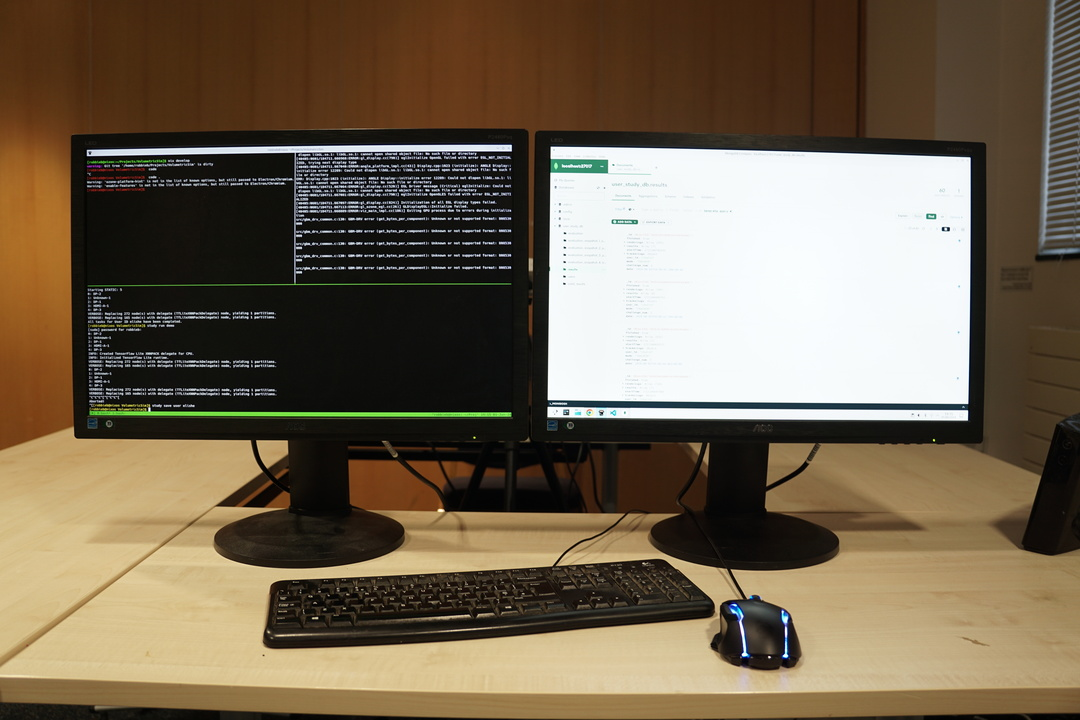
\includegraphics{./implementation/figures/control-view.jpg}
	  }
	}
	\hfill
	\pictureBox[label={fig:calibration-device-study}]{Study: Calibration Device}{
	\adjustbox{height=5cm, keepaspectratio}{
	  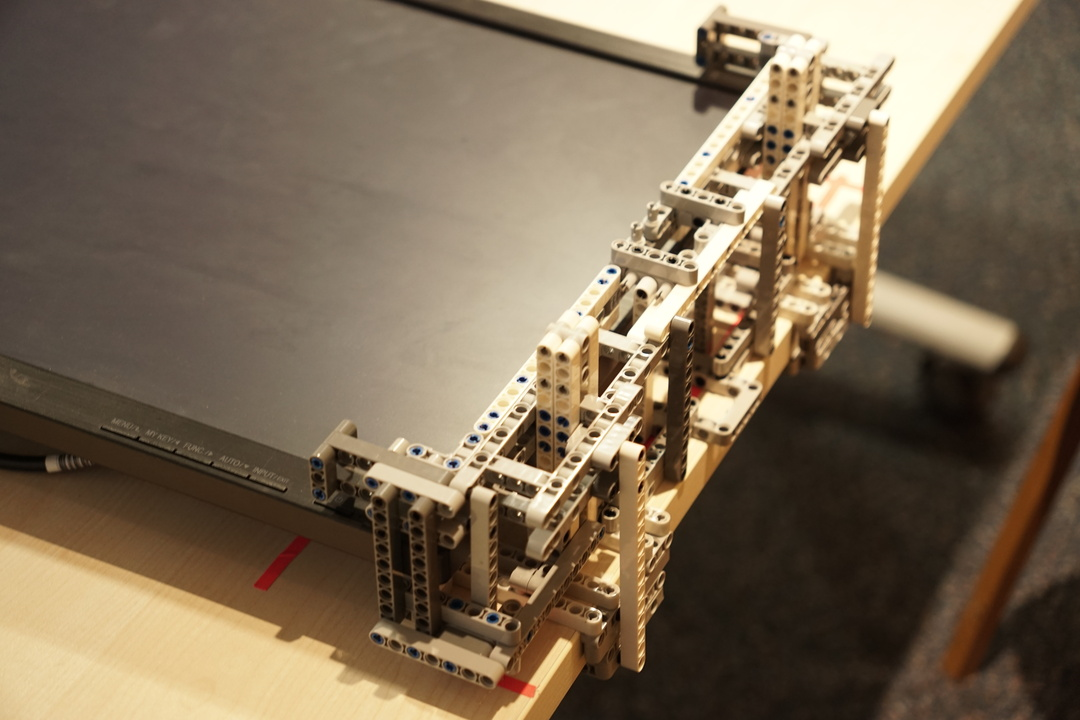
\includegraphics{./implementation/figures/calibration-device.jpg}
	  }
	}
\end{invisBox}

we also created a calibration device that can be seen in Fig~\ref{fig:calibration-device-study} to re-align the displays. This was a simple device made from Lego Technic \tocite that allowed us to easily re-align the displays if they were knocked out of place by the participants during the study.

\subsection{Evaluation Metrics and Collected Data}
The evaluation metrics we used to evaluate the system were primarily the time taken to complete the task and the number of subtasks completed. We took a time stamp at the beginning of each task and at the end of each subtask. \\

We also logged through the task the position of the participants eye, and hand coupled with time stamps to allow us to analyse the data in more detail. This allowed us to visually plot the paths participants as can be seen in Fig~\ref{fig:finger-trace}. \\


\begin{figureBox}[label={fig:finger-trace}, width=0.8\linewidth]{Example of logging a users path for Task 4}
    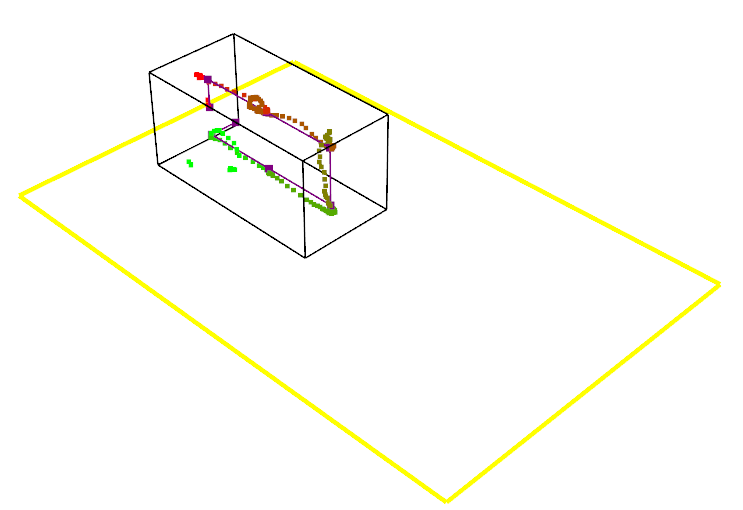
\includegraphics[width = 0.8\linewidth]{./implementation/figures/finger-trace-plot.png}
\end{figureBox}

\textcolor{red}{picture of consent form, put the whole survey in the appendix}

\subsection{Study Implementation}

The study was run from a python based CLI using the Click library. The simulator was compiled as a shared library and called from the python CLI using a C-FFI (foreign function interface). The results and logs were received from python in json format and stored in a mongoDB database.

\textcolor{red}{if have time include code CLI snippet, draw basic diagram with mongodb?}
